\documentclass[11pt,oneside,a4paper]{article}
\usepackage{graphicx}
\usepackage{hyperref}
\usepackage{float}
\usepackage{amsmath}

\title{Strace in XV6}
\author{Xiang Mei \\ \href{mailto:xm2146@nyu.edu}{xm2146@nyu.edu} }

\begin{document}
\maketitle
\section{Introduction}

\begin{figure}[H]
    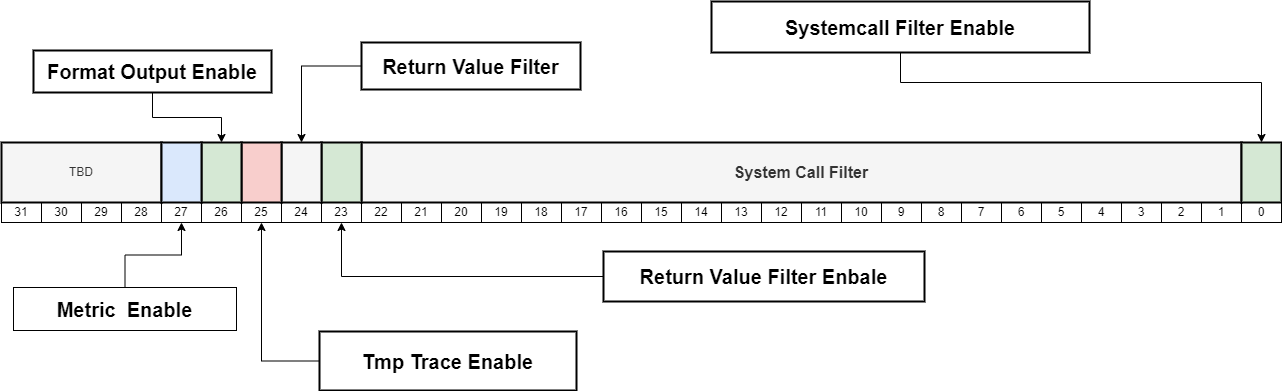
\includegraphics[width=4.75in]{pstrace.png}
    \centering
    \caption{My Strace}
\end{figure}

Strace is a very useful tool on Linux. It's widely used to do the troubleshooting.
But we don't have pre-installed strace on XV6. I'll implement a simple strace on XV6.

It sounds like reinventing a wheel. But for my expeirence in this course, Intro to OS,
I think write a simple version of "wheel" could help me to understand the
complesity of the "wheel" and help me think as an engineer. We need to consider
about lots of questions during the implementation, such as "why should the wheel be 
round?". Anyway, I learned a lot and used some skills I learn from previous assignment.

The first section is the introduction of the report and I'll document my design in the
second section. The real task-related parts start from the section 3.

\section{Get familiar with Linux strace}
In order to get familiar with the real strace, I use it to trace the sleep command.
After reading the help page of strace, I use the "-C" flag to show the list of called
syscalls, total number of calls, time of running strace on command.

\begin{figure}[H]
    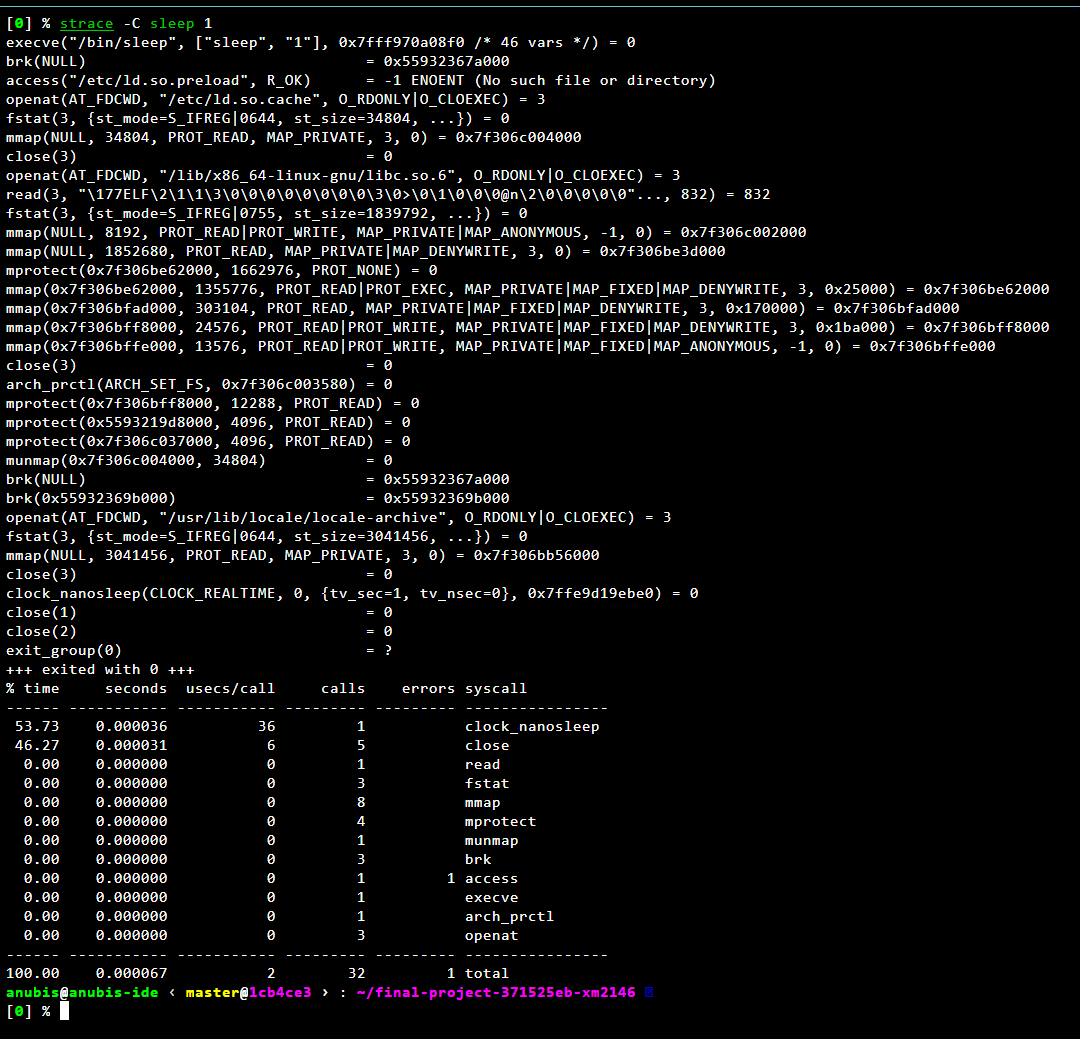
\includegraphics[width=4.75in]{1-3.png}
    \centering
    \caption{Task 1-1}
\end{figure}

For task 1-2, I choose "mmap, read, execve, mprotect" as the targets to explain. We can
see the procedure clearly on above figure. The "execve" call is called once and 
that's the first syscall we called. The "sleep" is an executable file in our system
and the execve syscall could run it. It's worthy to mention the executed binary would 
use the caller's memory space and proc struct. By the way, the execve syscall has three
3 parameters, the first one is the path of the executable binary. And the second one
would store the arguments while the third one would store the enviroment parameters.


The mmap syscall is used to allocate a large chunk of memory. In our command, 
it's used to allocate memory to store the shared libraries, the linker and other 
needed files. As we can see in above figure, mmap is usually called after openat.
The first parameter of mmap syscall is the address of the allocated chunk. You can 
set it NULL to represent arbitrary address and we can also set it a non-NULL value
to get a chunk strat from that adddress. This is used to allocate more space based 
on known chunk. The second parameter is the length we want to allocate while the thrid
arguments is the permission of the chunk, such as readable, writeable, and executeable.

And the mprotect is used  to change the permission of memory. The mprotect can't 
allocate new memory. It could only change the permission of the memory chunks. 
In our command, it's used to make mmaped memory not writeable. For example, we 
allocate a chunk for the shared libraries and the memory must be writeable because
we need copy the bytecodes to the memory. But you know it's dangerous to make writeable
memory executable. So we need mprotect to make it un-writeable after copying.

The syscall read is kind of straitforward. It reads the content from the first parameter's
corresponding file and store to the second parameter's correctly memory while the third
parameter is the max length of content the read syscall could read. It's used once to 
read the header of our glibc.

So far, we go through the usage and the shown information of strace on linux.
Strace is a useful tools and I have been using it for a long time but I still 
find something new by reading it's help page. And we are going to implement 
out strace.

\section{What features do we need}

In this assignment, we gonna implement a simple strace. I'll go through and features 
needed. 

For my implementation, the command should be like:

\begin{figure}[H]
    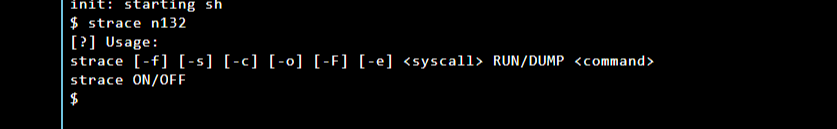
\includegraphics[width=4.75in]{1-4.png}
    \centering
    \caption{Usage}
\end{figure}

We have 4 sub-commands("RUN", "DUMP", "ON", and "OFF"), 3 filter options("-e","-s",and "-f"),
and 3 output control options("-F","-c", and "-o").

I'll introduce these options and sub-commands in later section. And there are a short 
version introduction: The sub-command "RUN" could strace the following command and 
trace the syscall until the following command exits and the "DUMP" would dump the 
syscall records in the kernel. Also we can use "strace on" to ask the kernel keeps
recording syscalls while the "strace off" could get the kernel back to the normal mode.

If we add "-e" options, the strace would only record and print specific syscalls. 
Besides, "-s/f" flag would force the strace to only record and print successful/failed
syscalls. 

Moreover, we have output control options. The "-F" flag would print more readable 
output and the "-c" would print a table of syscall metrics. As for "-o", it can set 
an output file and the strace's output would be stored in that file.

\section{Design}

This section will tell you the reasons of my design. 
This time, not like the "uniq" assignment, our implementation is different 
from the real sample because we don't have pthread syscall in xv6. Also, the 
strace is a big project I don't have much time to read its code. So during the 
implementation, I try to solve the problem myself and look up the matrials when 
I don't have an elegant solution.

\paragraph*{ON/OFF}

\begin{quotation}
    "When typing 'strace on' in the terminal, the mode of strace is on and therefore the next type in
command will be traced. The system call list will be printed on screen in format pid (process id),
command name, system call name, return value."
\end{quotation}
The "ON/OFF" implementation is easy and straitforward. In the requirements, we need
to print the pid, name, and syscall of processes. Obviously, we can't do this task
in userspace. I create an global variable in kernel space to present current 
strace\_mode.
\begin{figure}[H]
    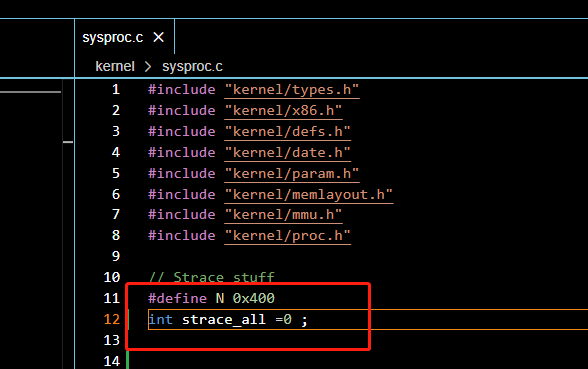
\includegraphics[width=4.75in]{1-5.png}
    \centering
    \caption{Strace All}
\end{figure}
Like what shows in the above figure, I set a global variable in "sysproc.c" because I'll
later implement a syscall as a bridge to stransfer command from user space to the kernel.

\begin{figure}[H]
    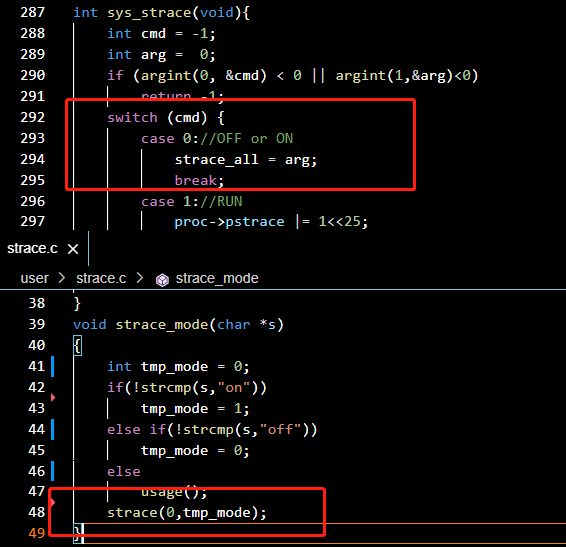
\includegraphics[width=4.75in]{1-6.png}
    \centering
    \caption{Strace Syscall}
\end{figure}
As you can see in the above figure, I parse the parameters from the command line and 
use strace syscall to modify the kernel variable. Basically, we can use the code above
to control the strace mode from user space. Nevertheless, how do we monitor the 
syscalls.

At very first, a simple plan came up in my mind: I can insert a piece of code in every
syscall so that I can print the result and parameters when running the syscall. 
And I use a global variable "strace\_all" to tell the system if we should print the
strace info while calling syscalls. But quickly I found there are some serious 
issues with this solution. We have 21 syscalls and if we need to write different 
strace\_handle for every syscall and it's not convinience because we may need to 
modify 21 places for every single change. My expeirence told me it's horriable. 
We must implement something more elegant.

The advantage of the previous plan is that we can print the arguments of syscalls.
If we need to print the content of the syscall we have to do that because the 
syscalls would parse the parameters in these syscall handlers. I asked in slack 
and found we don't need to print the details about the syscall so that we can
move the strace code to the syscall\_interupt handle or the wrapper function.

\begin{figure}[H]
    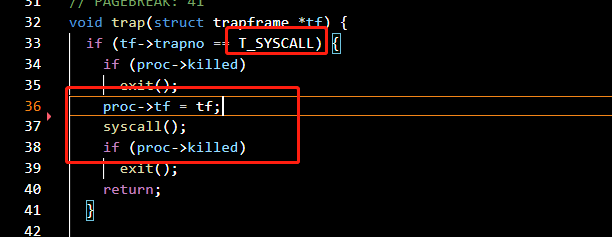
\includegraphics[width=4.75in]{1-1.png}
    \centering
    \caption{Syscall Handler in Trap Fcuntion}
\end{figure}

As we talked in this trap section, the syscall in user space would use create an
interupt to inform the kernel. And the interup is handled by the function alltraps 
in "trapasm.S" it would store current context in the trap frame and call function 
trap which is shown on the above figure. And we can see the trap would check the 
process's state and call the function syscall. This function is in file syscall.c.

\begin{figure}[H]
    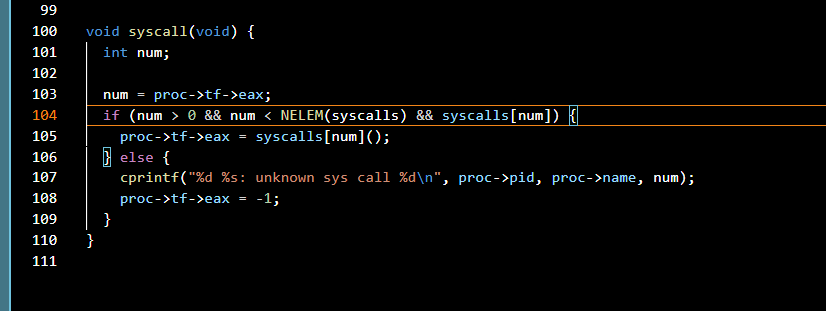
\includegraphics[width=4.75in]{1-2.png}
    \centering
    \caption{Syscall Wrapper}
\end{figure}

In this function, we would parse the EAX which represent the syscall index and 
store the return value in the EAX. So I think this function is a good candidate
to insert our strace code. 

\begin{figure}[H]
    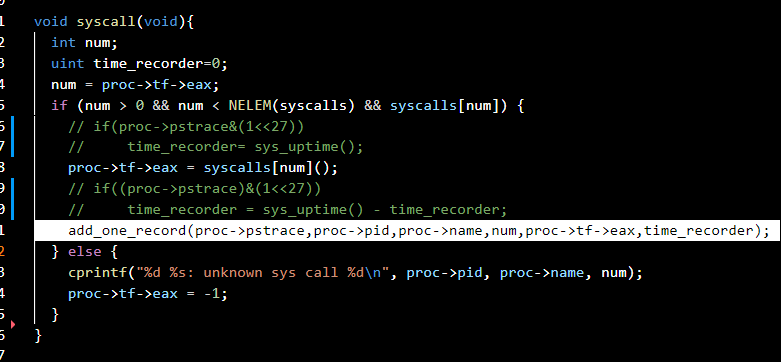
\includegraphics[width=4.75in]{1-7.png}
    \centering
    \caption{Monitor}
\end{figure}

I insert the monitor after the syscall because we need the return value the syscall
but we may loss "exit" syscall because the process would stop in "exit" syscall. 
So I add the same function before the process really exits which is shown in the figure 9.

\begin{figure}[H]
    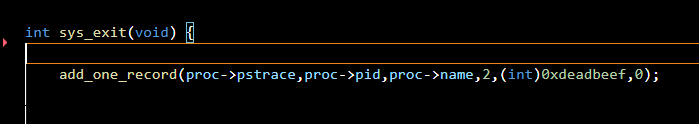
\includegraphics[width=4.75in]{1-8.png}
    \centering
    \caption{Strace Handler in sys\_exit}
\end{figure}

The usage of this sub-command is simple. You can just use "strace on" to turn on
strace and "strace off" to turn off strace.

\begin{figure}[H]
    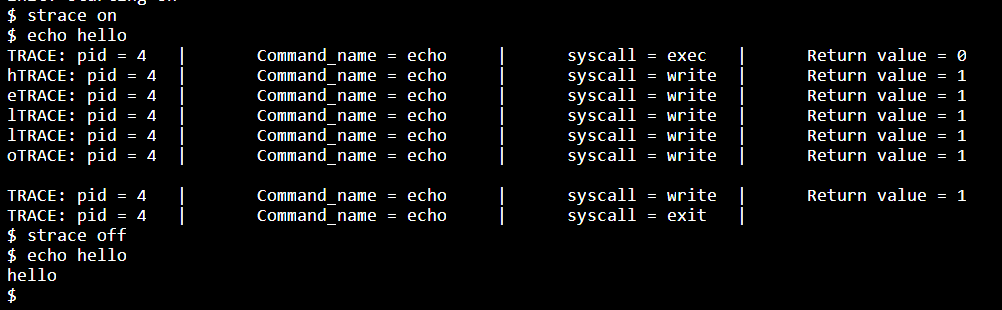
\includegraphics[width=4.75in]{1-13.png}
    \centering
    \caption{Strace On and OFF}
\end{figure}

There is no thing more about these 
two sub-commands but there is little problem about the global variable. In order for 
avoiding race condition, we need to implement lock mechanism for this variable. Howerver,
this not the requirement for this assignment and there is only one member in my team. 
I decide to do implement that only if I have time left.




\paragraph*{DUMP}
\begin{quotation}
"Implement a kernel memory that will save N number of latest events. This N number can be
configurable by using define in XV6. In order word, it can be hard code but the way to implement
is to use define to declare a variable called N with certain value. When 'strace dump' command is
called, print all events that saved in kernel memory."
\end{quotation}
In previosu figures, you may noticed that I implemented a function to log the syscall.
so why do I implement a such conplex function "add\_one\_record".

For implementing the "DUMP" feature, we need to allocate a space in the kernel to store
the latest N system calls. These data have to be stored in the kernel space as a global 
variable because xv6 is a multi-process system. And we need a special circle buffer to
store latest N records.

\begin{figure}[H]
    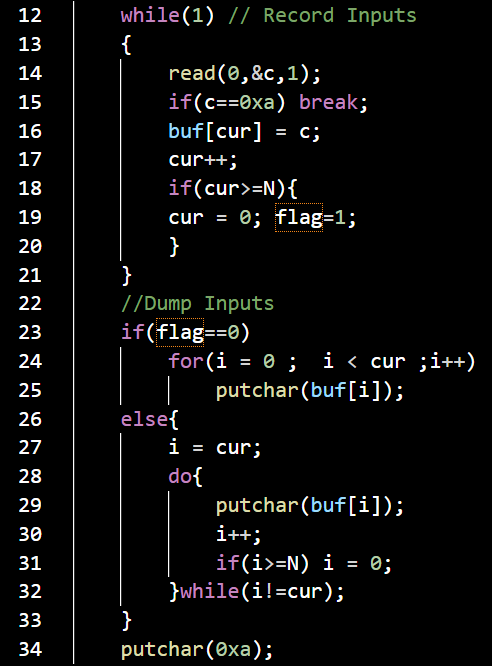
\includegraphics[width=4.75in]{1-9.png}
    \centering
    \caption{Circle Buffer}
\end{figure}

Circle buffer for DUMP operation is easier than general circle buffer. First, I 
implemented a C code version for testing. As you can see in the above figure, 
We read the input to the circle buffer and dump the content when we get an "enter".
The read-part is simple and the "flag" variable is important. It decides how many
and where to dump. The trick in the code is simple and makes sure we would print the
last N records which is veried by my fuzzer. That's another reason why I write it 
in C. Also, I attach my fuzz code:

\begin{figure}[H]
    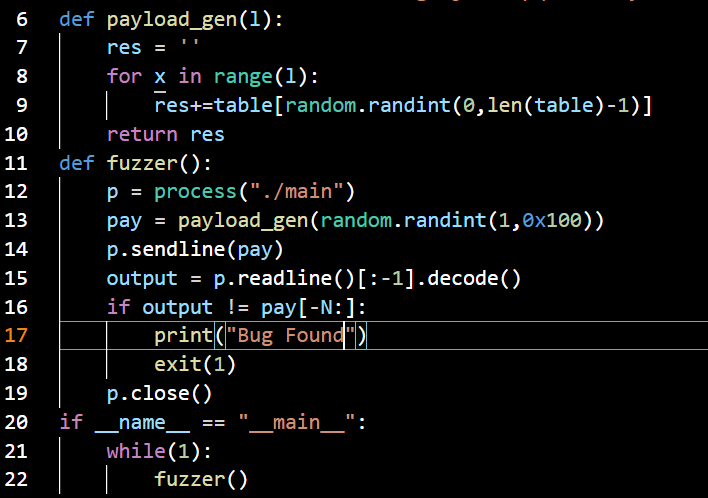
\includegraphics[width=4.75in]{1-10.png}
    \centering
    \caption{Circle Buffer Fuzzer}
\end{figure}

After other testing, I implement a similar circle buffer in the kernel to store and 
dump the syscalls. In function "add\_one\_record", I record the syscall's inform in 
the correct node and move the pointer like what I did in my previous demo. 

\begin{figure}[H]
    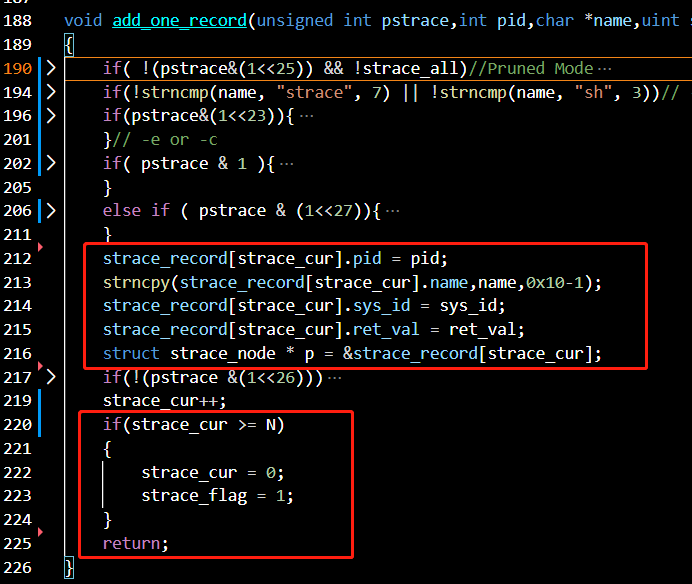
\includegraphics[width=4.75in]{1-11.png}
    \centering
    \caption{Circle Buffer Fuzzer}
\end{figure}

That's the key function of all my design I'll metion this function later to introduce 
otehr features. This function is only called in function syscall and sys\_exit so that
if we want to modify, delete, or add a feature to strace, we can just modify the code 
in this function. Another advantage is that we can naturally combine kinds of options.

\begin{figure}[H]
    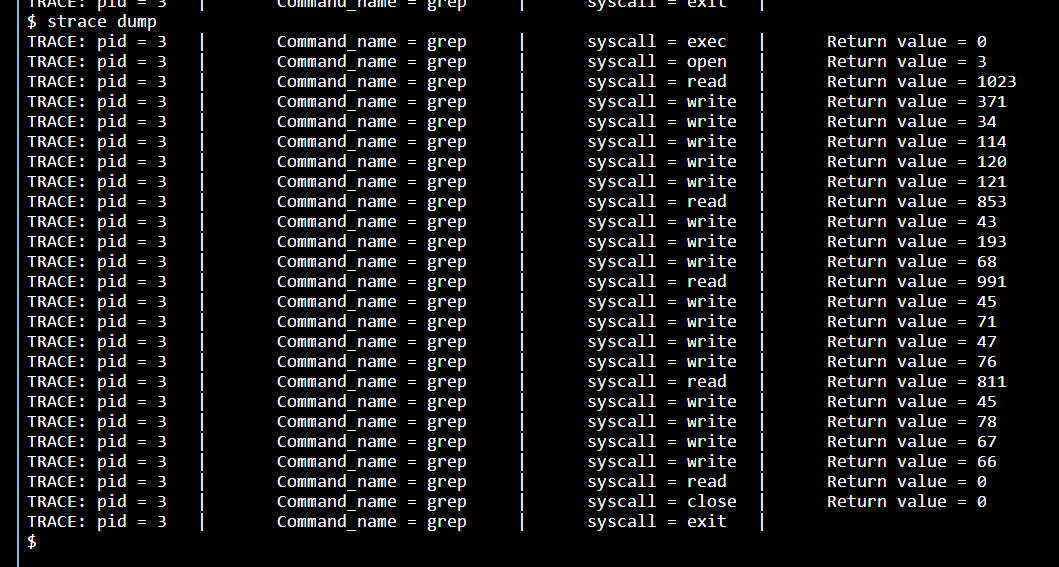
\includegraphics[width=4.75in]{1-12.png}
    \centering
    \caption{DUMP after Traing "grep the readme.md"}
\end{figure}

I did several tests on DUMP and it works well. I attach a simple sample above because 
the output of complex testcase would be big and hard to recognize. 
You can also test it with any commands you like and please check the README.md file 
attached to the assignment submission.

\paragraph*{RUN}

\begin{quotation}
    "Instead of turning on and off strace, we create 'strace run' to directly point tracing to the current
process that execute the command. For example: when typing 'strace run echo hello' in the
terminal, we get the output tracing of echo hello."
\end{quotation}

For sub-command "RUN", we gonna run a command and strace the syscall of the command.
So we can parse the parameter and use "fork" or "exec" syscall to run the command.

I used the "exec" syscall for my strace and there is a disadvantage comparing with 
the fork version. I know the fork version from my professor: 
we can use "fork" to creat a child process and let the parent process wait for the 
metadata of outputs from the kernel. So all the output part would be handledin user 
space which is much more secure and beautiful. Howerver, I almost finish my implementation
and there is no much time for this huge modification. Therefore, I'll keep my "exec"
version and for my implementation I think they are similar on complesity.


\begin{figure}[H]
    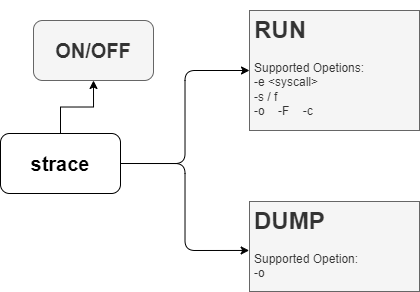
\includegraphics[width=4.75in]{1-14.png}
    \centering
    \caption{Supported Opetions}
\end{figure}

The "RUN" sub-command is the most complex part of my strace, I'll introduce some 
basic idea about this sub-command in this parameter and explain the rest parts with
the supported options. So how can we strace one command once?

If we "RUN" a command, we are going to use "fork" to create a new process or use 
"exec" to run a executable file by using current memory space. We must have a way to 
pass the information that the new process shoud be traced. In order to implement this,
I add a new element in "proc" struct in proc.

\begin{figure}[H]
    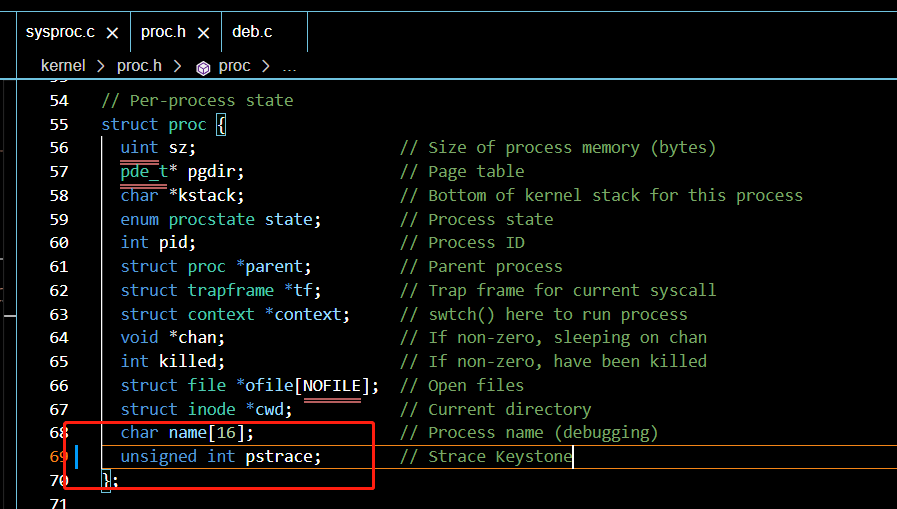
\includegraphics[width=4.75in]{1-15.png}
    \centering
    \caption{Strace a Process}
\end{figure}

As you can see in the above figure, I add a unsigned interger to the proc struct.
I don't want to wast unnecessary space in the kernel space.
so I would use this 4 bytes variable to store all the strace information such as 
output filter information and output format information. I'll explain the struct of
this variable in option-related paragraph.

\begin{figure}[H]
    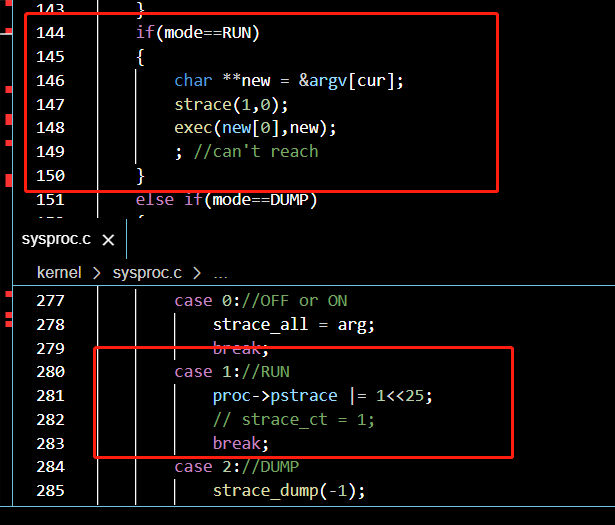
\includegraphics[width=4.00in]{1-16.png}
    \centering
    \caption{RUN Sub-command in User Space}
\end{figure}

The above figure is my userspace interface and corresponding system call implementation.
As you can see I use the 26th bit of the "pstrace" to sign if the kernel should strace
the process. Another advantage of having a variable in the "proc" struc is that we can 
easily follow the subprocess by modify the "fork" function in "proc.c".

\begin{figure}[H]
    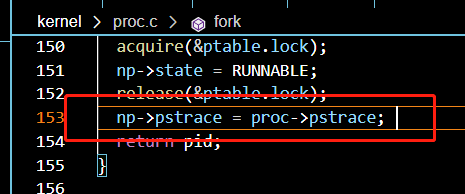
\includegraphics[width=4.00in]{1-17.png}
    \centering
    \caption{Trace the Child Processes}
\end{figure}

Now we can use strace to run strace any process! There is a simple demo of "RUN" 
sub-command.

\begin{figure}[H]
    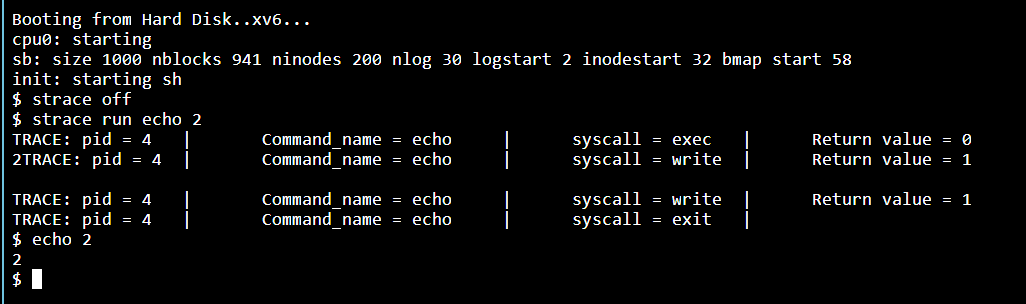
\includegraphics[width=4.75in]{1-18.png}
    \centering
    \caption{Strace RUN}
\end{figure}

\paragraph*{Opetions}

\begin{quotation}
    Our strace supports kinds of output filter and format options which could help to 
eliminate the uninterested sycalls. 
\end{quotation}

\begin{figure}[H]
    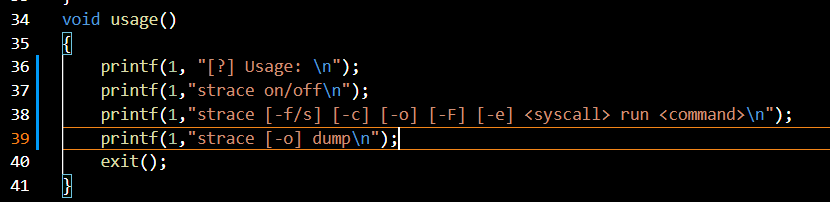
\includegraphics[width=4.75in]{1-19.png}
    \centering
    \caption{Supported Opetions}
\end{figure}




\end{document}